\section{Introduction}
\label{sec:intro}

Compositional generalization --- the ability to interpret novel combinations of known
primitives --- is a longstanding test for sequence-to-sequence models.
SCAN \citep{lake2018scan} is a standard benchmark: a model trained on primitive commands
must generalize those primitives to compound forms not seen in training.
T5-small \citep{raffel2020t5} fine-tuned on the \texttt{add\_prim\_jump} split must
learn the novel primitive \texttt{jump} from primitive-only training examples and apply
it correctly to compound commands.

At the checkpoint studied here (S-043), T5-small achieves low training loss but fails
on 56.8\% of compound-jump test commands (4376/7706).
The encoder marks \texttt{jump} as categorically distinct from trained primitives
($p=0.0000$, Mann--Whitney), so the failure occurs despite encoder awareness of the
out-of-distribution (OOD) primitive.
This paper asks: where exactly does the failure occur, what mechanism produces it, and
can a targeted weight-level intervention partially repair it?

\subsection{The Failure Mode}

The dominant failure is \emph{substituted-walk}: T5 generates
$(\texttt{I\_TURN\_LEFT}\ \texttt{I\_WALK}){\times}4$ when the correct output is
$(\texttt{I\_TURN\_LEFT}\ \texttt{I\_JUMP}){\times}4$.
The cycle count is correct; the cycle structure is correct; only the action token is wrong.
T5 has learned the four-cycle identity morphism for \texttt{around} commands but cannot
fill the action slot with the OOD primitive.

The failure is structurally concentrated.
Commands containing \texttt{around} fail at 87.3\% versus 22.4\% without it
(lift $+0.648$, AUC$=0.806$, $\chi^2$~$p=0.0000$, S-047).
At the action-slot divergence step, decoder cross-attention routing to the \texttt{around}
encoder position shows no detected difference between fail and success cases
($p=0.9208$, S-049): the decoder is looking at the right encoder position.
The failure emerges downstream of routing, in what the decoder reads back from the
attended position.
Figure~\ref{fig:failure-rate} shows the per-feature failure rate breakdown.

\begin{figure}[t]
\centering
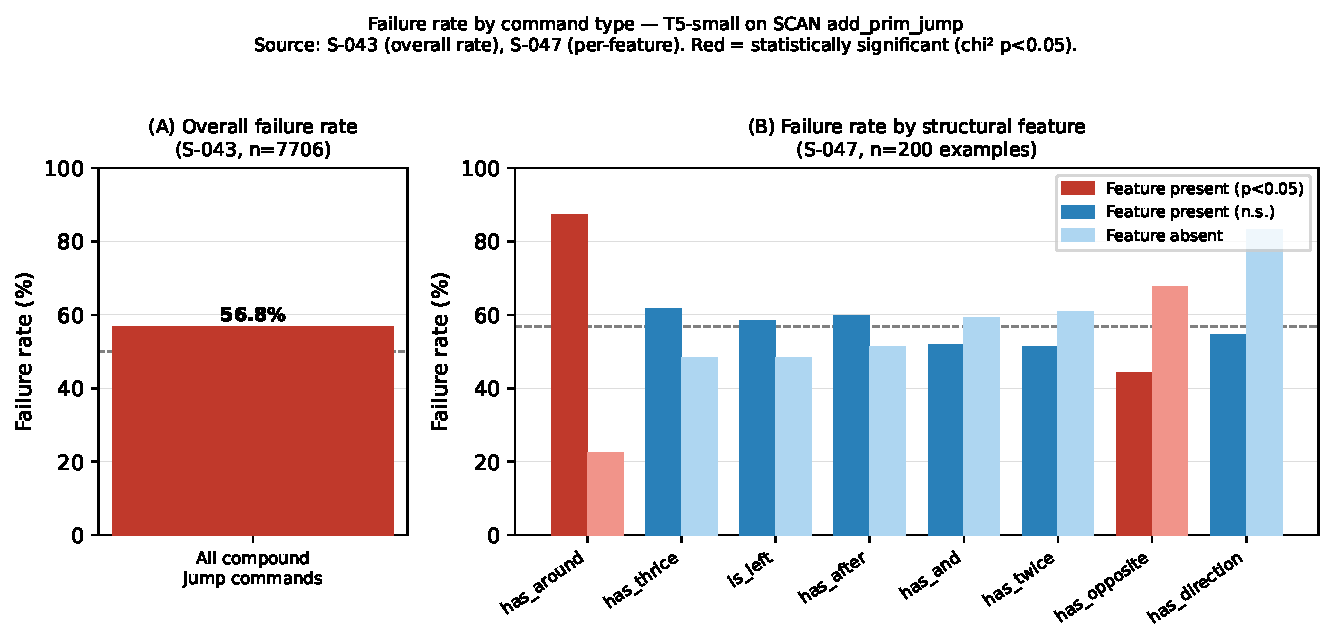
\includegraphics[width=\linewidth]{figures/fig01_failure_rate_by_command_type}
\caption{Failure rate by structural command feature. T5-small fine-tuned on SCAN
\texttt{add\_prim\_jump} (S-043 checkpoint). Overall failure rate 56.8\% on
compound-jump test set ($n=7706$). Per-feature breakdown from S-047 ($n=200$
examples). Red bars: statistically significant ($\chi^2$~$p < 0.05$).
\texttt{has\_around} is the dominant failure predictor (lift $+0.648$, AUC$=0.806$).}
\label{fig:failure-rate}
\end{figure}

\subsection{\texorpdfstring{The Locate $\to$ Explain $\to$ Repair Chain}{The Locate to Explain to Repair Chain}}

This paper reports a three-stage mechanistic account of one substituted-walk failure
mode in one T5-small checkpoint.

\paragraph{Locate (\S\S\ref{sec:locating}).}
Value-direction evidence identifies two decoder cross-attention heads, L4H6 and L5H5,
that attend strongly to the \texttt{jump} encoder token but contribute in the
\texttt{I\_WALK} direction at the action slot (S-051; confirmed in logit decomposition
S-059b).
Cross-attention routing is not the primary discriminator in the stored comparison
($p=0.9208$, S-049); the failure occurs in the value projection, not in where the
decoder looks.

\paragraph{Explain (\S\ref{sec:explaining}).}
Two mechanisms account for the output.
First, the cross-attention total at the action slot pushes $-171.25$ logit units toward
\texttt{I\_WALK}; FFN/embedding correction pushes $+165.25$ units back, leaving a net
margin of $-6.005$: near-cancellation with a $28.52\times$ reconstruction fraction
(S-059b).
Second, output embedding norm asymmetry ($\|\texttt{I\_WALK}\|\approx 520$ versus
$\|\texttt{I\_JUMP}\|\approx 424$) amplifies this small pro-walk residual to extreme
probabilities ($P(\texttt{I\_WALK})=0.914$ in fail cases); equalizing the norms
collapses this to $0.323$ (S-051 Option~A).

\paragraph{Repair (\S\ref{sec:repair}).}
A rank-1 modification to $W_V$ at L4H6 and L5H5 --- redirecting the mapping of the OOD
\texttt{jump} encoder representation from a pro-walk to a pro-jump value direction ---
improves the fail-group logit margin in every arm at every tested $\alpha$ value.
At $\alpha=1.0$, the joint correction shifts the mean fail margin by $+2.902$ logit units
and flips 16/30 sampled failures, using a perturbation of approximately 8\% of each
head's $W_V$ Frobenius norm (S-061).
The dose-response is monotonically linear.

A parallel controlled geometry track (G-track, \S\ref{sec:phase-diagram}) demonstrates
the same structural phenomena --- near-cancellation divergence, value-direction
substitution, and a causal/diagnostic head distinction --- in a transparent NumPy
toy model where all parameters are designed.
The G-track is a structural reference, not a calibrated predictor of T5-small behavior.

\subsection{Contributions}

\begin{enumerate}
  \item \textbf{Locate/explain/repair chain for a selected T5-small failure.}
    A closed three-stage account of the substituted-walk failure mode, from structural
    localization through mechanistic explanation to a weight-level intervention at the
    predicted site (\S\S\ref{sec:locating}--\ref{sec:repair}).
    This bounded mechanistic account is the paper's primary contribution.

  \item \textbf{Near-cancellation plus norm-asymmetry account.}
    Cross-attention and FFN contributions nearly cancel ($28.52\times$ reconstruction
    fraction); the small residual is amplified to dominant probabilities by output
    embedding norm asymmetry.
    The norm lever is identified as the primary amplifier (S-051 Option~A).

  \item \textbf{Rank-1 $W_V$ repair with monotonic dose-response.}
    A surgical weight-level correction that improves the fail-group margin in the
    predicted direction with a perturbation of ${\approx}8\%$ Frobenius norm and no OOD
    collapse across any tested configuration.

  \item \textbf{Two-track methodology.}
    A parallel production/toy design in which S-track and G-track independently
    exhibit near-cancellation and value substitution.
    Structural convergence across architectures, not calibrated quantitative prediction,
    is the claimed relationship.

  \item \textbf{Born filter instrument.}
    A controlled-geometry per-head Beck--Chevalley defect measurement used in the
    G-track to identify collapse conditions, phase regimes, and the causal/diagnostic
    head distinction (\S\ref{sec:phase-diagram}).
    In this paper the Born filter functions as a controlled reference model and
    supporting diagnostic framework, not as the primary evidence for the T5-small repair.
\end{enumerate}

\subsection{What This Paper Does Not Claim}

\begin{itemize}
  \item \textbf{Universal repair.}
    The rank-1 $W_V$ correction improves 16/30 sampled fail examples.
    14 examples do not flip, and the mean fail margin remains pro-walk after the
    intervention.
    The repair is partial and has been tested on one sampled group.

  \item \textbf{Broad specificity.}
    Success-group regression was tested on $n=2$ examples (S-062).
    Whether the correction affects commands that do not involve the \texttt{jump}
    encoder direction (\texttt{walk around}, \texttt{run around}, \texttt{look around})
    is not established.

  \item \textbf{All compositional failures are $W_V$ failures.}
    The value-projection account is established for the substituted-walk failure mode
    in \texttt{has\_around}=1 commands at this checkpoint.
    Other SCAN failure modes, other OOD primitives, and other model architectures
    may involve different mechanisms.

  \item \textbf{G-track as proof of the T5-small mechanism.}
    G-track results are established in controlled NumPy geometry with engineered
    embeddings.
    The G-track Born filter ratios, phase-diagram thresholds, and gamma-sweep values
    are not calibrated to T5-small logit magnitudes.
    The relationship is structural analogy, not quantitative prediction.
\end{itemize}

\subsection{Code and Reproducibility}

The companion workbench for this paper is available at
\url{https://github.com/mpe-framework/glass-attention-workbench-reproducibility}.
It contains the available experiment scripts, sealed result records, figure-generation
code (each figure is regenerated from a committed CSV), the arXiv source manifest,
and reconstruction or follow-up stencils for the controls discussed in the paper.
Some late-stage experiments were developed in Google Colab and are committed as
Colab-oriented scripts; the repository marks these cases explicitly.
The unrun future controls referenced in \S\ref{sec:discussion} --- for example the
broader specificity test on non-\texttt{jump} \texttt{around} commands --- are provided
as stencils and are not part of the present paper's claims.
